Buvo nustatyta, kad testavimo duomenyse egzistuoja klasių išsibalansavimas, kuris matosi iš \ref{tbl:class_imbalance} lentelės. Tad tikslumo matas gali nekorektiškai įvertinti dirbtinių neuroninių tinklų rezultatus. Todėl vietoje tikslumo mato tolimesniuose tyrimuose yra renkamas mikro, makro ir svertinis F1 įverčio (angl. F1 score) matai, kurie geriau įvertina dirbtinius neuroninius tinklus esant klasių išsibalansavimui nei tikslumo matas. F1 įvertis yra apskaičiuojamas kiekvienai klasei atskirai naudojant formulę (\ref{eqn:f1}), kur:

\begin{itemize}
	\item $TP$ - teisingų teigiamų (angl. true positives) kiekis. Teisingi teigiami yra 3D objektai, kuriems dirbtinis neuroninis tinklas teisingai priskyrė klasę, kuriai yra skaičiuojamas F1.
	\item $FP$ - klaidingų teigiamų (angl. false positives) kiekis. Klaidingi teigiami yra 3D objektai, kuriems dirbtinis neuroninis tinklas klaidingai priskyrė klasę, kuriai yra skaičiuojamas F1.
	\item $FN$ - klaidingų neigiamų (angl. false negatives) kiekis. Klaidingi neigiami yra 3D objektai, kuriems dirbtinis neuroninis tinklas klaidingai nepriskyrė klasės, kuriai yra skaičiuojamas F1.
\end{itemize}

Jų vidurkis yra lygus makro F1 įverčiui. Toliau yra apskaičiuojamas svertinis vidurkis (angl. weighted average), kur svoriai yra 3D objektų su priskirta klase, kuriai yra apskaičiuotas F1, dalis testavimo duomenyse. Šis vidurkis yra lygus svertiniui F1 įverčiui. Galiausiai yra apskaičiuojamas mikro F1 įvertis. Mikro F1 įvertis yra apskaičiuojamas naudojant formulę \ref{eqn:f1}, kur $TP$ yra teisingų teigiamų suma, $FP$ - klaidingų teigiamų suma ir $FN$ - klaidingų neigiamų suma. F1 įverčių matai yra skaičiuojami tik testavimo duomenims.

\begin{equation}
\label{eqn:f1}
	F1 = \dfrac{TP}{TP + \dfrac{1}{2}(FP + FN)}
\end{equation}

\begin{table}[]
\caption{3D objektų skaičius kiekvienai klasei testavimo duomenyse}
\begin{tabular}{lr}
	klasė       &   3D objektų skaičius \\
	\hline
	airplane    &                    99 \\
	bathtub     &                    50 \\
	bed         &                   100 \\
	bench       &                    20 \\
	bookshelf   &                   100 \\
	bottle      &                   100 \\
	bowl        &                    20 \\
	car         &                    99 \\
	chair       &                    99 \\
	cone        &                    20 \\
	cup         &                    20 \\
	curtain     &                    20 \\
	desk        &                    86 \\
	door        &                    20 \\
	dresser     &                    86 \\
	flower\_pot  &                    20 \\
	glass\_box   &                   100 \\
	guitar      &                    99 \\
	keyboard    &                    20 \\
	lamp        &                    20 \\
	laptop      &                    20 \\
	mantel      &                   100 \\
	monitor     &                   100 \\
	night\_stand &                    86 \\
	person      &                    20 \\
	piano       &                   100 \\
	plant       &                   100 \\
	radio       &                    20 \\
	range\_hood  &                   100 \\
	sink        &                    20 \\
	sofa        &                   100 \\
	stairs      &                    20 \\
	stool       &                    20 \\
	table       &                   100 \\
	tent        &                    20 \\
	toilet      &                   100 \\
	tv\_stand    &                   100 \\
	vase        &                   100 \\
	wardrobe    &                    20 \\
	xbox        &                    20 \\
\end{tabular}
\label{tbl:class_imbalance}
\end{table}


Taip pat pastebėta iš \ref{img:val_plot} grafiko, kad kapsulinio ir daugiavaizdžių kapsulinių neuroninių tinklų tikslumas netampa stabilus po 10 epochų. Tačiau, dėl Kaggle sistemos kodo apdorojimo laiko limito, kuris yra 9 valandos, didesnis epochų skaičius nei 12 yra negalimas, nes 1 tyrimas su 12 epochų trunka apytiksliai 8,5 valandos. Tad visi tolimesni tyrimai yra  atlikti su 12 apmokymo epochų.

Tyrimų, kuriuose buvo renkamos f1 įverčio metrikos ir naudojama 12 apmokymo epochos, rezultatai yra atvaizduoti: lentelėje \ref{tbl:weighted_f1} ir grafike \ref{img:weighted_f1} - testavimo duomenų svertiniai f1 įverčiai apmokant su visais apmokymo duomenimis, lentelėje \ref{tbl:micro_f1} ir grafike \ref{img:micro_f1} - testavimo duomenų mikro f1 įverčiai apmokant su visais apmokymo duomenimis, lentelėje \ref{tbl:macro_f1} ir grafike \ref{img:macro_f1} - testavimo duomenų makro f1 įverčiai su apmokant visais apmokymo duomenimis, lentelėje \ref{tbl:half_sample_f1} ir grafike \ref{img:half_sample_f1} - testavimo duomenų f1 įverčiai apmokant su apmokymo duomenimis sudarytais iš 4904 3D objektų modelių, lentelėje \ref{tbl:3rd_sample_f1} ir grafike \ref{img:3rd_sample_f1} - testavimo duomenų f1 įverčiai apmokant su apmokymo duomenimis sudarytais iš 3264 3D objektų modelių, kur
mvcnn yra daugiavaizdžio neuroninio tinklo f1 įverčiai, capsnet - kapsulinio neuroninio tinklo f1 įverčiai, mv\_capsnet - daugiavaizdžio kapsulinio neuroninio tinklo su vaizdų sujungimo sluoksniu f1 įverčiai, mv\_cap\_capsnet1 - daugiavaizdžio kapsulinio neuroninio tinklo su vaizdų kapsuliniu sluoksniu ir vienu mokymosi etapu f1 įverčiai, mv\_cap\_capsnet2 - daugiavaizdžio kapsulinio neuroninio tinklo su vaizdų kapsuliniu sluoksniu ir dviem mokymosi etapais f1 įverčiai, 
mvcnn\_weighted -  daugiavaizdžio konvoliucinio neuroninio tinklo svertiniai f1 įverčiai, 
mvcnn\_micro -  daugiavaizdžio konvoliucinio neuroninio tinklo mikro f1 įverčiai, 
mvcnn\_macro -  daugiavaizdžio konvoliucinio neuroninio tinklo makro f1 įverčiai, 
mv\_cap\_capsnet\_1\_weighted - daugiavaizdžio kapsulinio neuroninio tinklo su vaizdų kapsuliniu sluoksniu ir vienu mokymosi etapu svertiniai f1 įverčiai, 
mv\_cap\_capsnet\_1\_micro - daugiavaizdžio kapsulinio neuroninio tinklo su vaizdų kapsuliniu sluoksniu ir vienu mokymosi etapu mikro f1 įverčiai ir
mv\_cap\_capsnet\_1\_macro - daugiavaizdžio kapsulinio neuroninio tinklo su vaizdų kapsuliniu sluoksniu ir vienu mokymosi etapu makro f1 įverčiai. 
Brūkšninė vertikali linija grafikuose nurodo antrojo apmokymo etapo pirmąją epochą. Kiekviename stulpelyje geriausi pasiekti tikslumai yra paryškinti.

\begin{table}[]
	\caption{
		Testavimo duomenų klasifikavimo svertiniai f1 įverčiai, kur mvcnn yra daugiavaizdžio konvoliucinio neuroninio tinklo svertiniai f1 įverčiai, capsnet - kapsulinio neuroninio tinklo svertiniai f1 įverčiai, mv\_capsnet - daugiavaizdžio kapsulinio neuroninio tinklo su vaizdų sujungimo sluoksniu svertiniai f1 įverčiai, mv\_cap\_capsnet1 - daugiavaizdžio kapsulinio neuroninio tinklo su vaizdų kapsuliniu sluoksniu ir vienu mokymosi etapu svertiniai f1 įverčiai, mv\_cap\_capsnet2 - daugiavaizdžio kapsulinio neuroninio tinklo su vaizdų kapsuliniu sluoksniu ir dviem mokymosi etapais svertiniai f1 įverčiai. Kiekviename stulpelyje geriausi pasiekti tikslumai yra paryškinti.
	}
	\begin{tabular}{l|l|l|l|l|l}
		epocha & mvcnn & capsnet & mv-capsnet & mv-cap-capsnet1 & mv-cap-capsnet2 \\
		\hline
		1 & 0,807 &   0,703 &      0,653 &           0,606 &           0,541 \\
		2 & 0,836 &   0,769 &      0,760 &           0,780 &           0,722 \\
		3 & 0,853 &   0,768 &      0,796 &           0,797 &           0,778 \\
		4 & 0,852 &   0,784 &      0,801 &           0,827 &           0,786 \\
		5 & 0,862 &   0,792 &      0,819 &           0,838 &           0,810 \\
		6 & 0,851 &   0,790 &      0,824 &           0,839 &           0,815 \\
		7 & 0,881 &   0,795 &      0,788 &           0,838 &           0,811 \\
		8 & 0,892 &   0,795 &      0,799 &           0,852 &           0,844 \\
		9 & \textbf{0,908} &   0,795 &      0,810 &           0,848 &           0,851 \\
		10 & 0,885 &   0,788 &      0,805 &           0,852 &           0,854 \\
		11 & 0,897 &   \textbf{0,800} &      \textbf{0,827} &           \textbf{0,866} &           0,861 \\
		12 & 0,907 &   0,797 &      0,826 &           0,864 &           \textbf{0,861} \\
	\end{tabular}
	\label{tbl:weighted_f1}
\end{table}

\begin{table}[]
	\caption{
		Testavimo duomenų klasifikavimo mikro f1 įverčiai, kur mvcnn yra daugiavaizdžio konvoliucinio neuroninio tinklo mikro f1 įverčiai, capsnet - kapsulinio neuroninio tinklo mikro f1 įverčiai, mv\_capsnet - daugiavaizdžio kapsulinio neuroninio tinklo su vaizdų sujungimo sluoksniu mikro f1 įverčiai, mv\_cap\_capsnet1 - daugiavaizdžio kapsulinio neuroninio tinklo su vaizdų kapsuliniu sluoksniu ir vienu mokymosi etapu mikro f1 įverčiai, mv\_cap\_capsnet2 - daugiavaizdžio kapsulinio neuroninio tinklo su vaizdų kapsuliniu sluoksniu ir dviem mokymosi etapais mikro f1 įverčiai. Kiekviename stulpelyje geriausi pasiekti tikslumai yra paryškinti.
	}
	\begin{tabular}{l|l|l|l|l|l}
		epocha & mvcnn & capsnet & mv-capsnet & mv-cap-capsnet1 & mv-cap-capsnet2 \\
		\hline
		1 & 0,808 &   0,715 &      0,666 &           0,630 &           0,567 \\
		2 & 0,833 &   0,771 &      0,767 &           0,789 &           0,729 \\
		3 & 0,856 &   0,770 &      0,798 &           0,806 &           0,781 \\
		4 & 0,850 &   0,786 &      0,806 &           0,833 &           0,787 \\
		5 & 0,864 &   0,794 &      0,821 &           0,845 &           0,810 \\
		6 & 0,848 &   0,791 &      0,825 &           0,843 &           0,819 \\
		7 & 0,876 &   0,796 &      0,794 &           0,843 &           0,819 \\
		8 & 0,889 &   0,796 &      0,805 &           0,854 &           0,850 \\
		9 & \textbf{0,909} &   0,796 &      0,812 &           0,850 &           0,855 \\
		10 & 0,887 &   0,787 &      0,807 &           0,853 &           0,855 \\
		11 & 0,899 &  \textbf{ 0,801} &      0,828 &           \textbf{0,866} &           0,862 \\
		12 & 0,907 &   0,797 &      \textbf{0,829} &           0,864 &           \textbf{0,862} \\
	\end{tabular}
	\label{tbl:micro_f1}
\end{table}

\begin{table}[]
	\caption{
		Testavimo duomenų klasifikavimo makro f1 įverčiai, kur mvcnn yra daugiavaizdžio konvoliucinio neuroninio tinklo makro f1 įverčiai, capsnet - kapsulinio neuroninio tinklo makro f1 įverčiai, mv\_capsnet - daugiavaizdžio kapsulinio neuroninio tinklo su vaizdų sujungimo sluoksniu makro f1 įverčiai, mv\_cap\_capsnet1 - daugiavaizdžio kapsulinio neuroninio tinklo su vaizdų kapsuliniu sluoksniu ir vienu mokymosi etapu makro f1 įverčiai, mv\_cap\_capsnet2 - daugiavaizdžio kapsulinio neuroninio tinklo su vaizdų kapsuliniu sluoksniu ir dviem mokymosi etapais makro f1 įverčiai. Kiekviename stulpelyje geriausi pasiekti tikslumai yra paryškinti.
	}
	\begin{tabular}{l|l|l|l|l|l}
		epocha & mvcnn & capsnet & mv-capsnet & mv-cap-capsnet1 & mv-cap-capsnet2 \\
		\hline
		1 & 0,760 &   0,649 &      0,581 &           0,501 &           0,454 \\
		2 & 0,791 &   0,714 &      0,699 &           0,689 &           0,658 \\
		3 & 0,807 &   0,713 &      0,740 &           0,710 &           0,719 \\
		4 & 0,812 &   0,728 &      0,754 &           0,752 &           0,736 \\
		5 & 0,817 &   0,741 &      0,772 &           0,762 &           0,761 \\
		6 & 0,808 &   0,740 &      0,778 &           0,776 &           0,766 \\
		7 & 0,845 &   0,748 &      0,740 &           0,777 &           0,724 \\
		8 & 0,860 &   0,749 &      0,751 &           0,801 &           0,769 \\
		9 & \textbf{0,872} &   0,748 &      0,765 &           0,793 &           0,787 \\
		10 & 0,856 &   0,738 &      0,758 &           0,799 &           0,789 \\
		11 & 0,858 &   \textbf{0,753} &      0,778 &           \textbf{0,811} &           0,794 \\
		12 & 0,870 &   0,747 &      \textbf{0,779} &           0,806 &           \textbf{0,800} \\
	\end{tabular}
	\label{tbl:macro_f1}
\end{table}

% -----------------------------------------------------------------------------------------------------------------------

\begin{figure}[H]
	\centering
	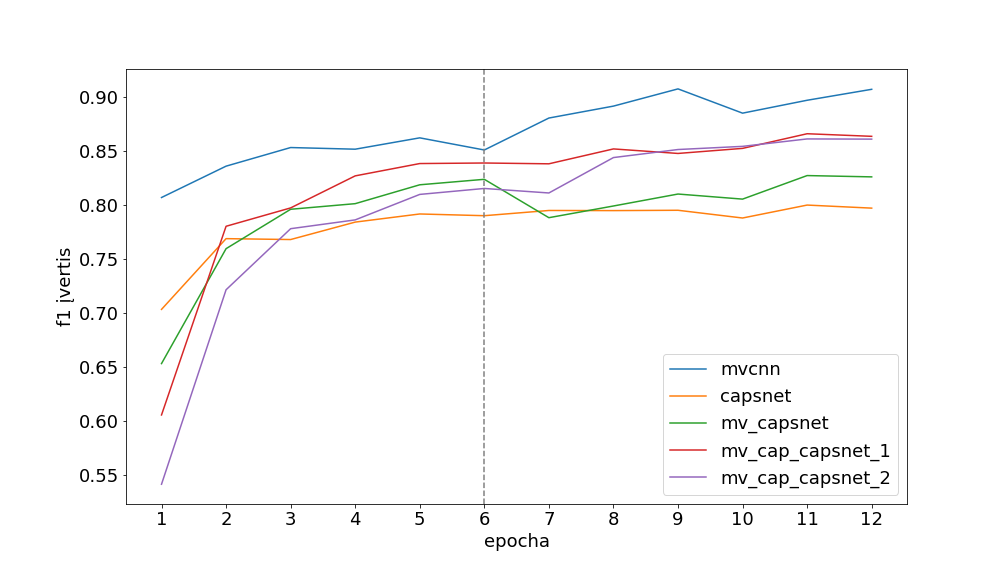
\includegraphics[scale=0.4]{img/weighted.png}
	\caption{
		Testavimo duomenų klasifikavimo svertiniai f1 įverčiai, kur mvcnn yra daugiavaizdžio konvoliucinio neuroninio tinklo svertiniai f1 įverčiai, capsnet - kapsulinio neuroninio tinklo svertiniai f1 įverčiai, mv\_capsnet - daugiavaizdžio kapsulinio neuroninio tinklo su vaizdų sujungimo sluoksniu svertiniai f1 įverčiai, mv\_cap\_capsnet1 - daugiavaizdžio kapsulinio neuroninio tinklo su vaizdų kapsuliniu sluoksniu ir vienu mokymosi etapu svertiniai f1 įverčiai, mv\_cap\_capsnet2 - daugiavaizdžio kapsulinio neuroninio tinklo su vaizdų kapsuliniu sluoksniu ir dviem mokymosi etapais svertiniai f1 įverčiai. Brūkšninė vertikali linija nurodo antrojo apmokymo etapo pirmąją epochą.
	}
	\label{img:weighted_f1}
\end{figure}

\begin{figure}[H]
	\centering
	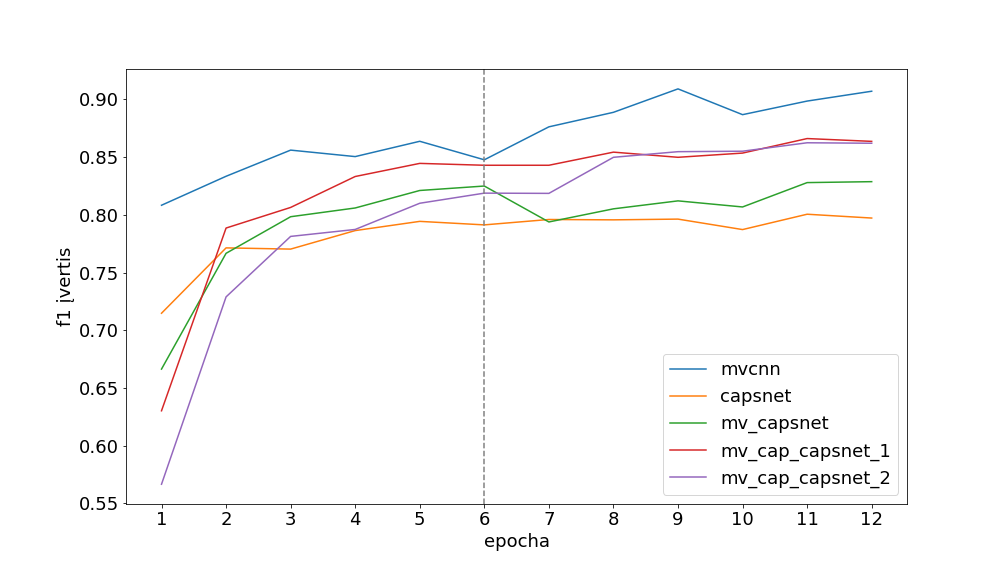
\includegraphics[scale=0.4]{img/micro.png}
	\caption{
		Testavimo duomenų klasifikavimo mikro f1 įverčiai, kur mvcnn yra daugiavaizdžio konvoliucinio neuroninio tinklo mikro f1 įverčiai, capsnet - kapsulinio neuroninio tinklo mikro f1 įverčiai, mv\_capsnet - daugiavaizdžio kapsulinio neuroninio tinklo su vaizdų sujungimo sluoksniu mikro f1 įverčiai, mv\_cap\_capsnet1 - daugiavaizdžio kapsulinio neuroninio tinklo su vaizdų kapsuliniu sluoksniu ir vienu mokymosi etapu mikro f1 įverčiai, mv\_cap\_capsnet2 - daugiavaizdžio kapsulinio neuroninio tinklo su vaizdų kapsuliniu sluoksniu ir dviem mokymosi etapais mikro f1 įverčiai. Brūkšninė vertikali linija nurodo antrojo apmokymo etapo pirmąją epochą.
	}
	\label{img:micro_f1}
\end{figure}

\begin{figure}[H]
	\centering
	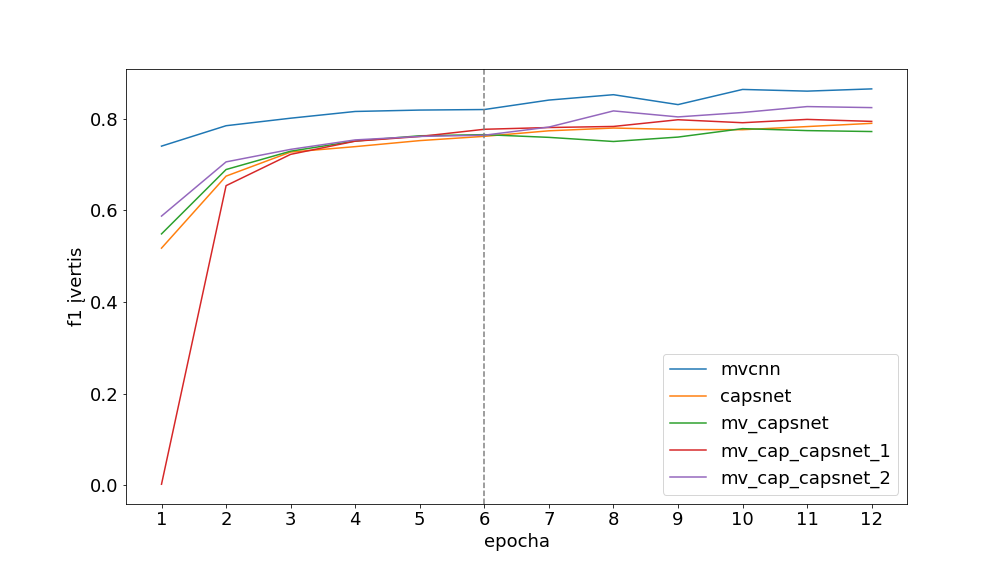
\includegraphics[scale=0.4]{img/macro.png}
	\caption{
		Testavimo duomenų klasifikavimo makro f1 įverčiai, kur mvcnn yra daugiavaizdžio konvoliucinio neuroninio tinklo makro f1 įverčiai, capsnet - kapsulinio neuroninio tinklo makro f1 įverčiai, mv\_capsnet - daugiavaizdžio kapsulinio neuroninio tinklo su vaizdų sujungimo sluoksniu makro f1 įverčiai, mv\_cap\_capsnet1 - daugiavaizdžio kapsulinio neuroninio tinklo su vaizdų kapsuliniu sluoksniu ir vienu mokymosi etapu makro f1 įverčiai, mv\_cap\_capsnet2 - daugiavaizdžio kapsulinio neuroninio tinklo su vaizdų kapsuliniu sluoksniu ir dviem mokymosi etapais makro f1 įverčiai. Brūkšninė vertikali linija nurodo antrojo apmokymo etapo pirmąją epochą.
	}
	\label{img:macro_f1}
\end{figure}

\begin{table}[]
	\caption{
		Tyrimų rezultatai su apmokymo duomenimis, sudarytais iš 4904 3D objektų modelių, kur mvcnn\_weighted -  daugiavaizdžio konvoliucinio neuroninio tinklo svertiniai f1 įverčiai, 
		mvcnn\_micro -  daugiavaizdžio konvoliucinio neuroninio tinklo mikro f1 įverčiai, 
		mvcnn\_macro -  daugiavaizdžio konvoliucinio neuroninio tinklo makro f1 įverčiai, 
		mv\_cap\_capsnet\_1\_weighted - daugiavaizdžio kapsulinio neuroninio tinklo su vaizdų kapsuliniu sluoksniu ir vienu mokymosi etapu svertiniai f1 įverčiai, 
		mv\_cap\_capsnet\_1\_micro - daugiavaizdžio kapsulinio neuroninio tinklo su vaizdų kapsuliniu sluoksniu ir vienu mokymosi etapu mikro f1 įverčiai ir
		mv\_cap\_capsnet\_1\_macro - daugiavaizdžio kapsulinio neuroninio tinklo su vaizdų kapsuliniu sluoksniu ir vienu mokymosi etapu makro f1 įverčiai. Kiekviename stulpelyje geriausi pasiekti tikslumai yra paryškinti.
	}
	\begin{tabular}{l|l|l|l|l|l|l}
		epocha & mvcnn\_weighted & mvcnn\_micro & mvcnn\_macro & \begin{tabular}[c]{@{}l@{}}mv\_cap\_1\\capsnet\\weighted\end{tabular} & \begin{tabular}[c]{@{}l@{}}mv\_cap\_1\\capsnet\\micro\end{tabular} & \begin{tabular}[c]{@{}l@{}}mv\_cap\_1\\capsnet\\macro\end{tabular} \\
		\hline
		1 &          0,723 &       0,731 &       0,661 &                     0,003 &                  0,026 &                  0,002 \\
		2 &          0,792 &       0,794 &       0,736 &                     0,598 &                  0,616 &                  0,488 \\
		3 &          0,810 &       0,805 &       0,755 &                     0,732 &                  0,743 &                  0,644 \\
		4 &          0,824 &       0,823 &       0,775 &                     0,781 &                  0,789 &                  0,700 \\
		5 &          0,828 &       0,828 &       0,782 &                     0,798 &                  0,804 &                  0,721 \\
		6 &          0,831 &       0,831 &       0,786 &                     0,800 &                  0,806 &                  0,720 \\
		7 &          0,845 &       0,845 &       0,810 &                     0,820 &                  0,825 &                  0,752 \\
		8 &          0,854 &       0,853 &       0,815 &                     0,824 &                  \textbf{0,828} &                  0,753 \\
		9 &          0,870 &       0,868 &       0,828 &                     \textbf{0,825} &                  0,827 &                  0,755 \\
		10 &          0,860 &       0,863 &       0,829 &                     0,817 &                  0,819 &                  0,748 \\
		11 &          \textbf{0,876} &       \textbf{0,875} &       0,833 &                     0,823 &                  0,823 &                  \textbf{0,756} \\
		12 &          0,872 &       0,871 &       \textbf{0,838} &                     0,821 &                  0,822 &                  0,754 \\
	\end{tabular}
	\label{tbl:half_sample_f1}
\end{table}

\begin{figure}[H]
	\centering
	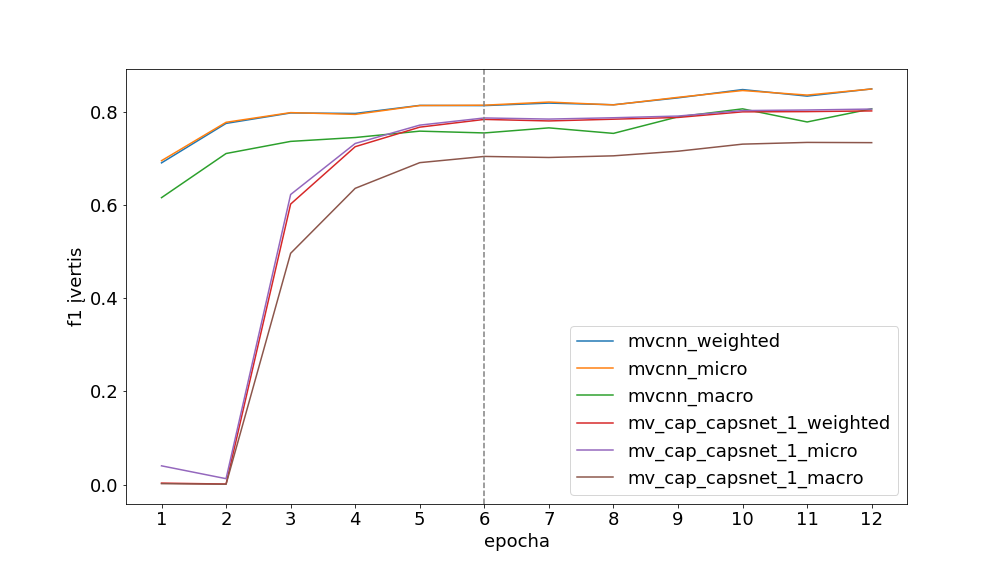
\includegraphics[scale=0.4]{img/half_sample_f1.png}
	\caption{
		Tyrimų rezultatai su apmokymo duomenimis, sudarytais iš 4904 3D objektų modelių, kur mvcnn\_weighted -  daugiavaizdžio konvoliucinio neuroninio tinklo svertiniai f1 įverčiai, 
		mvcnn\_micro -  daugiavaizdžio konvoliucinio neuroninio tinklo mikro f1 įverčiai, 
		mvcnn\_macro -  daugiavaizdžio konvoliucinio neuroninio tinklo makro f1 įverčiai, 
		mv\_cap\_capsnet\_1\_weighted - daugiavaizdžio kapsulinio neuroninio tinklo su vaizdų kapsuliniu sluoksniu ir vienu mokymosi etapu svertiniai f1 įverčiai, 
		mv\_cap\_capsnet\_1\_micro - daugiavaizdžio kapsulinio neuroninio tinklo su vaizdų kapsuliniu sluoksniu ir vienu mokymosi etapu mikro f1 įverčiai ir
		mv\_cap\_capsnet\_1\_macro - daugiavaizdžio kapsulinio neuroninio tinklo su vaizdų kapsuliniu sluoksniu ir vienu mokymosi etapu makro f1 įverčiai. Brūkšninė vertikali linija grafikuose nurodo antrojo apmokymo etapo pirmąją epochą.
	}
	\label{img:half_sample_f1}
\end{figure}

% -----------------------------------------------------------------------------------------------------------------------

\begin{table}[]
	\caption{
		Tyrimų rezultatai su apmokymo duomenimis, sudarytais iš 3264 3D objektų modelių, kur mvcnn\_weighted -  daugiavaizdžio konvoliucinio neuroninio tinklo svertiniai f1 įverčiai, 
		mvcnn\_micro -  daugiavaizdžio konvoliucinio neuroninio tinklo mikro f1 įverčiai, 
		mvcnn\_macro -  daugiavaizdžio konvoliucinio neuroninio tinklo makro f1 įverčiai, 
		mv\_cap\_capsnet\_1\_weighted - daugiavaizdžio kapsulinio neuroninio tinklo su vaizdų kapsuliniu sluoksniu ir vienu mokymosi etapu svertiniai f1 įverčiai, 
		mv\_cap\_capsnet\_1\_micro - daugiavaizdžio kapsulinio neuroninio tinklo su vaizdų kapsuliniu sluoksniu ir vienu mokymosi etapu mikro f1 įverčiai ir
		mv\_cap\_capsnet\_1\_macro - daugiavaizdžio kapsulinio neuroninio tinklo su vaizdų kapsuliniu sluoksniu ir vienu mokymosi etapu makro f1 įverčiai. Kiekviename stulpelyje geriausi pasiekti tikslumai yra paryškinti.
	}
	\begin{tabular}{l|l|l|l|l|l|l}
		epocha & mvcnn\_weighted & mvcnn\_micro & mvcnn\_macro & \begin{tabular}[c]{@{}l@{}}mv\_cap\_1\\capsnet\\weighted\end{tabular} & \begin{tabular}[c]{@{}l@{}}mv\_cap\_1\\capsnet\\micro\end{tabular} & \begin{tabular}[c]{@{}l@{}}mv\_cap\_1\\capsnet\\macro\end{tabular} \\
		\hline
		1 &          0,690 &       0,695 &       0,616 &                     0,003 &                  0,040 &                  0,002 \\
		2 &          0,775 &       0,778 &       0,711 &                     0,001 &                  0,013 &                  0,001 \\
		3 &          0,798 &       0,798 &       0,737 &                     0,602 &                  0,623 &                  0,496 \\
		4 &          0,797 &       0,795 &       0,745 &                     0,725 &                  0,732 &                  0,636 \\
		5 &          0,814 &       0,814 &       0,759 &                     0,767 &                  0,772 &                  0,691 \\
		6 &          0,813 &       0,814 &       0,755 &                     0,784 &                  0,787 &                  0,704 \\
		7 &          0,819 &       0,821 &       0,766 &                     0,780 &                  0,784 &                  0,702 \\
		8 &          0,815 &       0,815 &       0,754 &                     0,784 &                  0,787 &                  0,706 \\
		9 &          0,830 &       0,831 &       0,789 &                     0,788 &                  0,791 &                  0,716 \\
		10 &          0,848 &       0,846 &       0,806 &                     0,800 &                  0,803 &                  0,731 \\
		11 &          0,834 &       0,836 &       0,778 &                     0,801 &                  0,804 &                  0,734 \\
		12 &          \textbf{0,849} &       \textbf{0,849} &       \textbf{0,807} &                     \textbf{0,802} &                  \textbf{0,806} &                  \textbf{0,734} \\
	\end{tabular}
	\label{tbl:3rd_sample_f1}
\end{table}

\begin{figure}[H]
	\centering
	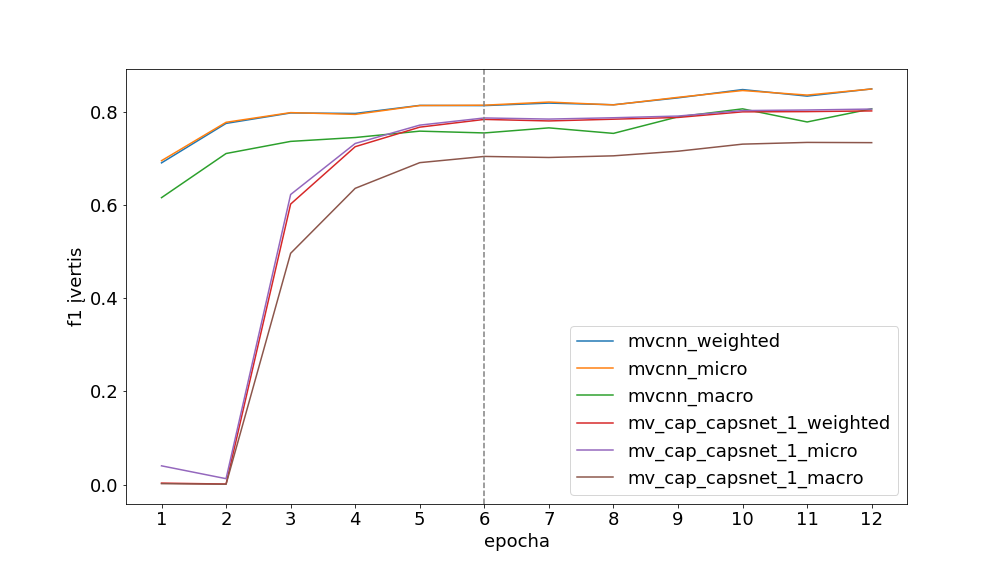
\includegraphics[scale=0.4]{img/3rd_sample_f1.png}
	\caption{
		Tyrimų rezultatai su apmokymo duomenimis, sudarytais iš 3264 3D objektų modelių, kur mvcnn\_weighted -  daugiavaizdžio konvoliucinio neuroninio tinklo svertiniai f1 įverčiai, 
		mvcnn\_micro -  daugiavaizdžio konvoliucinio neuroninio tinklo mikro f1 įverčiai, 
		mvcnn\_macro -  daugiavaizdžio konvoliucinio neuroninio tinklo makro f1 įverčiai, 
		mv\_cap\_capsnet\_1\_weighted - daugiavaizdžio kapsulinio neuroninio tinklo su vaizdų kapsuliniu sluoksniu ir vienu mokymosi etapu svertiniai f1 įverčiai, 
		mv\_cap\_capsnet\_1\_micro - daugiavaizdžio kapsulinio neuroninio tinklo su vaizdų kapsuliniu sluoksniu ir vienu mokymosi etapu mikro f1 įverčiai ir
		mv\_cap\_capsnet\_1\_macro - daugiavaizdžio kapsulinio neuroninio tinklo su vaizdų kapsuliniu sluoksniu ir vienu mokymosi etapu makro f1 įverčiai. Brūkšninė vertikali linija grafikuose nurodo antrojo apmokymo etapo pirmąją epochą.
	}
	\label{img:3rd_sample_f1}
\end{figure}

\ref{img:half_sample_f1} grafikas ir \ref{img:3rd_sample_f1} grafikas patvirtina įžvalgas padarytas iš \ref{img:less_datav1} grafiko ir \ref{img:less_datav2} grafiko. \ref{img:3rd_sample_f1} grafiko pirmų dvejų epochų rezultatai indikuoja prastus pradinius svorius. Tačiau tolimesnis apmokymas nusveria pradinių svorių įtaką.


% -----------------------------------------------------------------------------------------------------------------------
